% !TeX spellcheck = en_GB
\newgeometry{margin=1cm, top=2cm, bottom=2cm}
\section{Hecke Operators}
\subsection{Primes Hecke Operators}
\label{table:PrimeHeckeOperators}
\begin{center}
\begin{tabular}{|c|ccccccccccc|}
	\hline
	\textbf{} & \textbf{$\Delta^1$} & \textbf{$\Delta^3$} & \textbf{$\Delta^5$} & \textbf{$\Delta^7$} & \textbf{$\Delta^9$} & \textbf{$\Delta^{11}$} & \textbf{$\Delta^{13}$} & \textbf{$\Delta^{15}$} & \textbf{$\Delta^{17}$} & \textbf{$\Delta^{19}$} & \textbf{$\Delta^{21}$} \\\hline    
	$T_3$ & 0 & $\Delta^1$ & 0 & $\Delta^5$ & $\Delta^3$ & $\Delta^9$ & $\Delta^7$ & $\Delta^5 + \Delta^{13}$ & 0 & $\Delta^9 + \Delta^{17}$ & $\Delta^7$ \\
	$T_5$ & 0 & 0 & $\Delta^1$ & $\Delta^3$ & 0 & 0 & $\Delta^9$ & $\Delta^3 + \Delta^{11}$ & $\Delta^5$ & $\Delta^7$ & $\Delta^9 + \Delta^{17}$ 
	\\
	$T_7$ & 0 & 0 & 0 & $\Delta^1$ & 0 & 0 & $\Delta^3$ & $\Delta^9$ & 0 & $\Delta^5$ & $\Delta^3$ \\
	$T_{11}$ & 0 & $\Delta^1$ & 0 & $\Delta^5$ & $\Delta^3$ & $\Delta^1 + \Delta^9$ & $\Delta^7$ & $\Delta^{13}$ & 0 & $\Delta^9 + \Delta^{17}$ & $\Delta^7$ \\
	$T_{13}$ & 0 & 0 & $\Delta^1$ & $\Delta^3$ & 0 & 0 & $\Delta^1 + \Delta^9$ & $\Delta^{11}$ & $\Delta^5$ & $\Delta^7$ & $\Delta^9 + \Delta^{17}$ \\
	$T_{17}$ & 0 & 0 & 0 & 0 & $\Delta^1$ & $\Delta^3$ & $\Delta^5$ & $\Delta^7$ & $\Delta^1$ & 0 & 0 \\
	$T_{19}$ & 0 & $\Delta^1$ & 0 & $\Delta^5$ & $\Delta^3$ & $\Delta^1 + \Delta^9$ & $\Delta^7$ & $\Delta^{13}$ & 0 & $\Delta^1 + \Delta^9 + \Delta^{17}$ & $\Delta^7$ \\
	$T_{23}$ & 0 & 0 & 0 & $\Delta^1$ & 0 & 0 & $\Delta^3$ & $\Delta^1 + \Delta^9$ & 0 & $\Delta^5$ & $\Delta^3$ \\
	$T_{29}$ & 0 & 0 & $\Delta^1$ & $\Delta^3$ & 0 & 0 & $\Delta^9$ & $\Delta^3 + \Delta^{11}$ & $\Delta^5$ & $\Delta^7$ & $\Delta^1 + \Delta^9 + \Delta^{17}$ \\
	$T_{31}$ & 0 & 0 & 0 & 0 & 0 & 0 & 0 & $\Delta^1$ & 0 & 0 & 0 \\
	$T_{37}$ & 0 & 0 & $\Delta^1$ & $\Delta^3$ & 0 & 0 & $\Delta^1 + \Delta^9$ & $\Delta^{11}$ & $\Delta^5$ & $\Delta^7$ & $\Delta^9 + \Delta^{17}$ \\
	$T_{41}$ & 0 & 0 & 0 & 0 & 0 & 0 & 0 & 0 & $\Delta^1$ & $\Delta^3$ & $\Delta^5$ \\
	$T_{43}$ & 0 & $\Delta^1$ & 0 & $\Delta^5$ & $\Delta^3$ & $\Delta^9$ & $\Delta^7$ & $\Delta^5 + \Delta^{13}$ & 0 & $\Delta^9 + \Delta^{17}$ & $\Delta^7$ \\
	$T_{47}$ & 0 & 0 & 0 & 0 & 0 & 0 & 0 & $\Delta^1$ & 0 & 0 & 0 \\
	$T_{53}$ & 0 & 0 & $\Delta^1$ & $\Delta^3$ & 0 & 0 & $\Delta^1 + \Delta^9$ & $\Delta^{11}$ & $\Delta^5$ & $\Delta^7$ & $\Delta^1 + \Delta^9 + \Delta^{17}$ \\
	$T_{59}$ & 0 & $\Delta^1$ & 0 & $\Delta^5$ & $\Delta^3$ & $\Delta^9$ & $\Delta^7$ & $\Delta^5 + \Delta^{13}$ & 0 & $\Delta^1 + \Delta^9 + \Delta^{17}$ & $\Delta^7$ \\
	$T_{61}$ & 0 & 0 & $\Delta^1$ & $\Delta^3$ & 0 & 0 & $\Delta^1 + \Delta^9$ & $\Delta^{11}$ & $\Delta^5$ & $\Delta^7$ & $\Delta^1 + \Delta^9 + \Delta^{17}$ \\
	$T_{67}$ & 0 & $\Delta^1$ & 0 & $\Delta^5$ & $\Delta^3$ & $\Delta^1 + \Delta^9$ & $\Delta^7$ & $\Delta^{13}$ & 0 & $\Delta^9 + \Delta^{17}$ & $\Delta^7$ \\
	$T_{71}$ & 0 & 0 & 0 & $\Delta^1$ & 0 & 0 & $\Delta^3$ & $\Delta^1 + \Delta^9$ & 0 & $\Delta^5$ & $\Delta^3$ \\
	$T_{73}$ & 0 & 0 & 0 & 0 & $\Delta^1$ & $\Delta^3$ & $\Delta^5$ & $\Delta^7$ & 0 & $\Delta^3$ & $\Delta^5$ \\
	$T_{79}$ & 0 & 0 & 0 & 0 & 0 & 0 & 0 & 0 & 0 & 0 & 0 \\
	$T_{83}$ & 0 & $\Delta^1$ & 0 & $\Delta^5$ & $\Delta^3$ & $\Delta^9$ & $\Delta^7$ & $\Delta^5 + \Delta^{13}$ & 0 & $\Delta^1 + \Delta^9 + \Delta^{17}$ & $\Delta^7$ \\
	$T_{89}$ & 0 & 0 & 0 & 0 & $\Delta^1$ & $\Delta^3$ & $\Delta^5$ & $\Delta^7$ & 0 & $\Delta^3$ & $\Delta^5$ \\
	$T_{97}$ & 0 & 0 & 0 & 0 & $\Delta^1$ & $\Delta^3$ & $\Delta^5$ & $\Delta^7$ & $\Delta^1$ & 0 & 0 \\
	$T_{101}$ & 0 & 0 & $\Delta^1$ & $\Delta^3$ & 0 & 0 & $\Delta^1 + \Delta^9$ & $\Delta^{11}$ & $\Delta^5$ & $\Delta^7$ & $\Delta^9 + \Delta^{17}$ \\
	$T_{103}$ & 0 & 0 & 0 & $\Delta^1$ & 0 & 0 & $\Delta^3$ & $\Delta^1 + \Delta^9$ & 0 & $\Delta^5$ & $\Delta^3$ \\
	$T_{107}$ & 0 & $\Delta^1$ & 0 & $\Delta^5$ & $\Delta^3$ & $\Delta^1 + \Delta^9$ & $\Delta^7$ & $\Delta^{13}$ & 0 & $\Delta^9 + \Delta^{17}$ 
	& $\Delta^7$ \\
	$T_{109}$ & 0 & 0 & $\Delta^1$ & $\Delta^3$ & 0 & 0 & $\Delta^9$ & $\Delta^3 + \Delta^{11}$ & $\Delta^5$ & $\Delta^7$ & $\Delta^9 + \Delta^{17}$ \\
	$T_{113}$ & 0 & 0 & 0 & 0 & 0 & 0 & 0 & 0 & 0 & 0 & 0 \\
	$T_{127}$ & 0 & 0 & 0 & 0 & 0 & 0 & 0 & $\Delta^1$ & 0 & 0 & 0 \\
	$T_{131}$ & 0 & $\Delta^1$ & 0 & $\Delta^5$ & $\Delta^3$ & $\Delta^1 + \Delta^9$ & $\Delta^7$ & $\Delta^{13}$ & 0 & $\Delta^9 + \Delta^{17}$ 
	& $\Delta^7$ \\
	$T_{137}$ & 0 & 0 & 0 & 0 & 0 & 0 & 0 & 0 & $\Delta^1$ & $\Delta^3$ & $\Delta^5$ \\
	$T_{139}$ & 0 & $\Delta^1$ & 0 & $\Delta^5$ & $\Delta^3$ & $\Delta^9$ & $\Delta^7$ & $\Delta^5 + \Delta^{13}$ & 0 & $\Delta^9 + \Delta^{17}$ 
	& $\Delta^7$ \\
	$T_{149}$ & 0 & 0 & $\Delta^1$ & $\Delta^3$ & 0 & 0 & $\Delta^9$ & $\Delta^3 + \Delta^{11}$ & $\Delta^5$ & $\Delta^7$ & $\Delta^1 + \Delta^9 
	+ \Delta^{17}$ \\
	%	$T_{151}$ & 0 & 0 & 0 & $\Delta^1$ & 0 & 0 & $\Delta^3$ & $\Delta^1 + \Delta^9$ & 0 & $\Delta^5$ & $\Delta^3$ \\
	%	$T_{157}$ & 0 & 0 & $\Delta^1$ & $\Delta^3$ & 0 & 0 & $\Delta^1 + \Delta^9$ & $\Delta^{11}$ & $\Delta^5$ & $\Delta^7$ & $\Delta^1 + \Delta^9 
	%	+ \Delta^{17}$ \\
	%	$T_{163}$ & 0 & $\Delta^1$ & 0 & $\Delta^5$ & $\Delta^3$ & $\Delta^9$ & $\Delta^7$ & $\Delta^5 + \Delta^{13}$ & 0 & $\Delta^9 + \Delta^{17}$ 
	%	& $\Delta^7$ \\
	%	$T_{167}$ & 0 & 0 & 0 & $\Delta^1$ & 0 & 0 & $\Delta^3$ & $\Delta^9$ & 0 & $\Delta^5$ & $\Delta^3$ \\
	%	$T_{173}$ & 0 & 0 & $\Delta^1$ & $\Delta^3$ & 0 & 0 & $\Delta^1 + \Delta^9$ & $\Delta^{11}$ & $\Delta^5$ & $\Delta^7$ & $\Delta^9 + \Delta^{17}$ \\
	%	$T_{179}$ & 0 & $\Delta^1$ & 0 & $\Delta^5$ & $\Delta^3$ & $\Delta^9$ & $\Delta^7$ & $\Delta^5 + \Delta^{13}$ & 0 & $\Delta^1 + \Delta^9 + \Delta^{17}$ & $\Delta^7$ \\
	%	$T_{181}$ & 0 & 0 & $\Delta^1$ & $\Delta^3$ & 0 & 0 & $\Delta^9$ & $\Delta^3 + \Delta^{11}$ & $\Delta^5$ & $\Delta^7$ & $\Delta^1 + \Delta^9 
	%	+ \Delta^{17}$ \\
	%	$T_{191}$ & 0 & 0 & 0 & 0 & 0 & 0 & 0 & $\Delta^1$ & 0 & 0 & 0 \\
	%	$T_{193}$ & 0 & 0 & 0 & 0 & $\Delta^1$ & $\Delta^3$ & $\Delta^5$ & $\Delta^7$ & $\Delta^1$ & 0 & 0 \\
	%	$T_{197}$ & 0 & 0 & $\Delta^1$ & $\Delta^3$ & 0 & 0 & $\Delta^9$ & $\Delta^3 + \Delta^{11}$ & $\Delta^5$ & $\Delta^7$ & $\Delta^9 + \Delta^{17}$ \\
	%	$T_{199}$ & 0 & 0 & 0 & $\Delta^1$ & 0 & 0 & $\Delta^3$ & $\Delta^9$ & 0 & $\Delta^5$ & $\Delta^3$ \\
	\hline
\end{tabular}
Action of Primes Hecke Operators (primes up to $150$) on Modular Forms Modulo 2 (up to $\Delta^{21}$).
\end{center}

A larger table may be found \href{https://pauldubois98.github.io/ModularFormsModuloTwo.jl/tables/Hecke_primes_table.html}{online} at \url{https://pauldubois98.github.io/ModularFormsModuloTwo.jl/tables/Hecke_primes_table.html}.



\newgeometry{margin=0.5cm, top=1cm, bottom=2cm}
\subsection{Powers of Hecke Operators}
\label{table:PowersHeckeOperators}
\begin{center}
\begin{tabular}{|c|cccc|}
	\hline
	\textbf{$\Delta^1$} & \textbf{$T_5^0$} & \textbf{$T_5^1$} & \textbf{$T_5^2$} & \textbf{$\dots$} \\\hline
	$T_3^0$ & $\Delta^1$ & 0 & 0 & $\dots$ \\
	$T_3^1$ & 0 & 0 & 0 & $\dots$ \\
	$T_3^2$ & 0 & 0 & 0 & $\dots$ \\
	$\vdots$ & $\vdots$ & $\vdots$ & $\vdots$ & $\ddots$ \\\hline
\end{tabular}
\begin{tabular}{|c|cccc|}
	\hline
	\textbf{$\Delta^3$} & \textbf{$T_5^0$} & \textbf{$T_5^1$} & \textbf{$T_5^2$} & \textbf{$\dots$} \\\hline
	$T_3^0$ & $\Delta^3$ & 0 & 0 & $\dots$ \\
	$T_3^1$ & $\Delta^1$ & 0 & 0 & $\dots$ \\
	$T_3^2$ & 0 & 0 & 0 & $\dots$ \\
	$\vdots$ & $\vdots$ & $\vdots$ & $\vdots$ & $\ddots$ \\\hline
\end{tabular}
\begin{tabular}{|c|cccc|}
	\hline
	\textbf{$\Delta^5$} & \textbf{$T_5^0$} & \textbf{$T_5^1$} & \textbf{$T_5^2$} & \textbf{$\dots$} \\\hline
	$T_3^0$ & $\Delta^5$ & $\Delta^1$ & 0 & $\dots$ \\
	$T_3^1$ & 0 & 0 & 0 & $\dots$ \\
	$T_3^2$ & 0 & 0 & 0 & $\dots$ \\
	$\vdots$ & $\vdots$ & $\vdots$ & $\vdots$ & $\ddots$ \\\hline
\end{tabular}
\begin{tabular}{|c|cccc|}
	\hline
	\textbf{$\Delta^7$} & \textbf{$T_5^0$} & \textbf{$T_5^1$} & \textbf{$T_5^2$} & \textbf{$\dots$} \\\hline
	$T_3^0$ & $\Delta^7$ & $\Delta^3$ & 0 & $\dots$ \\
	$T_3^1$ & $\Delta^5$ & $\Delta^1$ & 0 & $\dots$ \\
	$T_3^2$ & 0 & 0 & 0 & $\dots$ \\
	$\vdots$ & $\vdots$ & $\vdots$ & $\vdots$ & $\ddots$ \\\hline
\end{tabular}
\begin{tabular}{|c|ccccc|}
	\hline
	\textbf{$\Delta^9$} & \textbf{$T_5^0$} & \textbf{$T_5^1$} & \textbf{$T_5^2$} & \textbf{$T_5^3$} & \textbf{$\dots$} \\\hline
	$T_3^0$ & $\Delta^9$ & 0 & 0 & 0 & $\dots$ \\
	$T_3^1$ & $\Delta^3$ & 0 & 0 & 0 & $\dots$ \\
	$T_3^2$ & $\Delta^1$ & 0 & 0 & 0 & $\dots$ \\
	$T_3^3$ & 0 & 0 & 0 & 0 & $\dots$ \\
	$\vdots$ & $\vdots$ & $\vdots$ & $\vdots$ & $\vdots$ & $\ddots$ \\\hline
\end{tabular}
\begin{tabular}{|c|ccccc|}
	\hline
	\textbf{$\Delta^{11}$} & \textbf{$T_5^0$} & \textbf{$T_5^1$} & \textbf{$T_5^2$} & \textbf{$T_5^3$} & \textbf{$\dots$} \\\hline
	$T_3^0$ & $\Delta^{11}$ & 0 & 0 & 0 & $\dots$ \\
	$T_3^1$ & $\Delta^9$ & 0 & 0 & 0 & $\dots$ \\
	$T_3^2$ & $\Delta^3$ & 0 & 0 & 0 & $\dots$ \\
	$T_3^3$ & $\Delta^1$ & 0 & 0 & 0 & $\dots$ \\
	$\vdots$ & $\vdots$ & $\vdots$ & $\vdots$ & $\vdots$ & $\ddots$ \\\hline
\end{tabular}
\begin{tabular}{|c|ccccc|}
	\hline
	\textbf{$\Delta^{13}$} & \textbf{$T_5^0$} & \textbf{$T_5^1$} & \textbf{$T_5^2$} & \textbf{$T_5^3$} & \textbf{$\dots$} \\\hline
	$T_3^0$ & $\Delta^{13}$ & $\Delta^9$ & 0 & 0 & $\dots$ \\
	$T_3^1$ & $\Delta^7$ & $\Delta^3$ & 0 & 0 & $\dots$ \\
	$T_3^2$ & $\Delta^5$ & $\Delta^1$ & 0 & 0 & $\dots$ \\
	$T_3^3$ & 0 & 0 & 0 & 0 & $\dots$ \\
	$\vdots$ & $\vdots$ & $\vdots$ & $\vdots$ & $\vdots$ & $\ddots$ \\\hline
\end{tabular}
\begin{tabular}{|c|cccccc|}
	\hline
	\textbf{$\Delta^{15}$} & \textbf{$T_5^0$} & \textbf{$T_5^1$} & \textbf{$T_5^2$} & \textbf{$T_5^3$} & \textbf{$T_5^4$} & \textbf{$\dots$} \\\hline
	$T_3^0$ & $\Delta^{15}$ & $\Delta^3 + \Delta^{11}$ & 0 & 0 & 0 & $\dots$ \\
	$T_3^1$ & $\Delta^5 + \Delta^{13}$ & $\Delta^1 + \Delta^9$ & 0 & 0 & 0 & $\dots$ \\
	$T_3^2$ & $\Delta^7$ & $\Delta^3$ & 0 & 0 & 0 & $\dots$ \\
	$T_3^3$ & $\Delta^5$ & $\Delta^1$ & 0 & 0 & 0 & $\dots$ \\
	$T_3^4$ & 0 & 0 & 0 & 0 & 0 & $\dots$ \\
	$\vdots$ & $\vdots$ & $\vdots$ & $\vdots$ & $\vdots$ & $\vdots$ & $\ddots$ \\\hline
\end{tabular}
\begin{tabular}{|c|cccccc|}
	\hline
	\textbf{$\Delta^{17}$} & \textbf{$T_5^0$} & \textbf{$T_5^1$} & \textbf{$T_5^2$} & \textbf{$T_5^3$} & \textbf{$T_5^4$} & \textbf{$\dots$} \\\hline
	$T_3^0$ & $\Delta^{17}$ & $\Delta^5$ & $\Delta^1$ & 0 & 0 & $\dots$ \\
	$T_3^1$ & 0 & 0 & 0 & 0 & 0 & $\dots$ \\
	$T_3^2$ & 0 & 0 & 0 & 0 & 0 & $\dots$ \\
	$T_3^3$ & 0 & 0 & 0 & 0 & 0 & $\dots$ \\
	$T_3^4$ & 0 & 0 & 0 & 0 & 0 & $\dots$ \\
	$\vdots$ & $\vdots$ & $\vdots$ & $\vdots$ & $\vdots$ & $\vdots$ & $\ddots$ \\\hline
\end{tabular}
\begin{tabular}{|c|cccccc|}
	\hline
	\textbf{$\Delta^{19}$} & \textbf{$T_5^0$} & \textbf{$T_5^1$} & \textbf{$T_5^2$} & \textbf{$T_5^3$} & \textbf{$T_5^4$} & \textbf{$\dots$} \\\hline
	$T_3^0$ & $\Delta^{19}$ & $\Delta^7$ & $\Delta^3$ & 0 & 0 & $\dots$ \\
	$T_3^1$ & $\Delta^9 + \Delta^{17}$ & $\Delta^5$ & $\Delta^1$ & 0 & 0 & $\dots$ \\
	$T_3^2$ & $\Delta^3$ & 0 & 0 & 0 & 0 & $\dots$ \\
	$T_3^3$ & $\Delta^1$ & 0 & 0 & 0 & 0 & $\dots$ \\
	$T_3^4$ & 0 & 0 & 0 & 0 & 0 & $\dots$ \\
	$\vdots$ & $\vdots$ & $\vdots$ & $\vdots$ & $\vdots$ & $\vdots$ & $\ddots$ \\\hline
\end{tabular}
\begin{tabular}{|c|cccccc|}
	\hline
	\textbf{$\Delta^{21}$} & \textbf{$T_5^0$} & \textbf{$T_5^1$} & \textbf{$T_5^2$} & \textbf{$T_5^3$} & \textbf{$T_5^4$} & \textbf{$\dots$} \\\hline
	$T_3^0$ & $\Delta^{21}$ & $\Delta^9 + \Delta^{17}$ & $\Delta^5$ & $\Delta^1$ & 0 & $\dots$ \\
	$T_3^1$ & $\Delta^7$ & $\Delta^3$ & 0 & 0 & 0 & $\dots$ \\
	$T_3^2$ & $\Delta^5$ & $\Delta^1$ & 0 & 0 & 0 & $\dots$ \\
	$T_3^3$ & 0 & 0 & 0 & 0 & 0 & $\dots$ \\
	$T_3^4$ & 0 & 0 & 0 & 0 & 0 & $\dots$ \\
	$\vdots$ & $\vdots$ & $\vdots$ & $\vdots$ & $\vdots$ & $\vdots$ & $\ddots$ \\\hline
\end{tabular}
\begin{tabular}{|c|cccccc|}
	\hline
	\textbf{$\Delta^{23}$} & \textbf{$T_5^0$} & \textbf{$T_5^1$} & \textbf{$T_5^2$} & \textbf{$T_5^3$} & \textbf{$T_5^4$} & \textbf{$\dots$} \\
	\hline
	$T_3^0$ & $\Delta^{23}$ & $\Delta^{11} + \Delta^{19}$ & $\Delta^7$ & $\Delta^3$ & 0 & $\dots$ \\
	$T_3^1$ & $\Delta^{13} + \Delta^{21}$ & $\Delta^{17}$ & $\Delta^5$ & $\Delta^1$ & 0 & $\dots$ \\
	$T_3^2$ & 0 & 0 & 0 & 0 & 0 & $\dots$ \\
	$T_3^3$ & 0 & 0 & 0 & 0 & 0 & $\dots$ \\
	$T_3^4$ & 0 & 0 & 0 & 0 & 0 & $\dots$ \\
	$\vdots$ & $\vdots$ & $\vdots$ & $\vdots$ & $\vdots$ & $\vdots$ & $\ddots$ \\
	\hline
\end{tabular}
\begin{tabular}{|c|cccccc|}
	\hline
	\textbf{$\Delta^{25}$} & \textbf{$T_5^0$} & \textbf{$T_5^1$} & \textbf{$T_5^2$} & \textbf{$T_5^3$} & \textbf{$T_5^4$} & \textbf{$\dots$} \\
	\hline
	$T_3^0$ & $\Delta^{25}$ & $\Delta^5 + \Delta^{13}$ & $\Delta^1 + \Delta^9$ & 0 & 0 & $\dots$ \\
	$T_3^1$ & $\Delta^{11} + \Delta^{19}$ & $\Delta^7$ & $\Delta^3$ & 0 & 0 & $\dots$ \\
	$T_3^2$ & $\Delta^{17}$ & $\Delta^5$ & $\Delta^1$ & 0 & 0 & $\dots$ \\
	$T_3^3$ & 0 & 0 & 0 & 0 & 0 & $\dots$ \\
	$T_3^4$ & 0 & 0 & 0 & 0 & 0 & $\dots$ \\
	$\vdots$ & $\vdots$ & $\vdots$ & $\vdots$ & $\vdots$ & $\vdots$ & $\ddots$ \\
	\hline
\end{tabular}
\begin{tabular}{|c|cccccc|}
	\hline
	\textbf{$\Delta^{27}$} & \textbf{$T_5^0$} & \textbf{$T_5^1$} & \textbf{$T_5^2$} & \textbf{$T_5^3$} & \textbf{$T_5^4$} & \textbf{$\dots$} \\
	\hline
	$T_3^0$ & $\Delta^{27}$ & $\Delta^7 + \Delta^{15}$ & $\Delta^{11}$ & 0 & 0 & $\dots$ \\
	$T_3^1$ & $\Delta^9 + \Delta^{17} + \Delta^{25}$ & $\Delta^{13}$ & $\Delta^9$ & 0 & 0 & $\dots$ \\
	$T_3^2$ & $\Delta^3 + \Delta^{11} + \Delta^{19}$ & $\Delta^7$ & $\Delta^3$ & 0 & 0 & $\dots$ \\
	$T_3^3$ & $\Delta^1 + \Delta^{17}$ & $\Delta^5$ & $\Delta^1$ & 0 & 0 & $\dots$ \\
	$T_3^4$ & 0 & 0 & 0 & 0 & 0 & $\dots$ \\
	$\vdots$ & $\vdots$ & $\vdots$ & $\vdots$ & $\vdots$ & $\vdots$ & $\ddots$ \\
	\hline
\end{tabular}
\begin{tabular}{|c|cccccc|}
	\hline
	\textbf{$\Delta^{29}$} & \textbf{$T_5^0$} & \textbf{$T_5^1$} & \textbf{$T_5^2$} & \textbf{$T_5^3$} & \textbf{$T_5^4$} & \textbf{$\dots$} \\
	\hline
	$T_3^0$ & $\Delta^{29}$ & $\Delta^{17} + \Delta^{25}$ & $\Delta^{13}$ & $\Delta^9$ & 0 & $\dots$ \\
	$T_3^1$ & $\Delta^{23}$ & $\Delta^{11} + \Delta^{19}$ & $\Delta^7$ & $\Delta^3$ & 0 & $\dots$ \\
	$T_3^2$ & $\Delta^{13} + \Delta^{21}$ & $\Delta^{17}$ & $\Delta^5$ & $\Delta^1$ & 0 & $\dots$ \\
	$T_3^3$ & 0 & 0 & 0 & 0 & 0 & $\dots$ \\
	$T_3^4$ & 0 & 0 & 0 & 0 & 0 & $\dots$ \\
	$\vdots$ & $\vdots$ & $\vdots$ & $\vdots$ & $\vdots$ & $\vdots$ & $\ddots$ \\
	\hline
\end{tabular}
%\begin{tabular}{|c|cccccc|}
%	\hline
%	\textbf{$\Delta^{31}$} & \textbf{$T_5^0$} & \textbf{$T_5^1$} & \textbf{$T_5^2$} & \textbf{$T_5^3$} & \textbf{$T_5^4$} & \textbf{$\dots$} \\
%	\hline
%	$T_3^0$ & $\Delta^{31}$ & $\Delta^{27}$ & $\Delta^7 + \Delta^{15}$ & $\Delta^{11}$ & 0 & $\dots$ \\
%	$T_3^1$ & $\Delta^{13} + \Delta^{29}$ & $\Delta^9 + \Delta^{17} + \Delta^{25}$ & $\Delta^{13}$ & $\Delta^9$ & 0 & $\dots$ \\
%	$T_3^2$ & $\Delta^7 + \Delta^{23}$ & $\Delta^3 + \Delta^{11} + \Delta^{19}$ & $\Delta^7$ & $\Delta^3$ & 0 & $\dots$ \\
%	$T_3^3$ & $\Delta^5 + \Delta^{13} + \Delta^{21}$ & $\Delta^1 + \Delta^{17}$ & $\Delta^5$ & $\Delta^1$ & 0 & $\dots$ \\
%	$T_3^4$ & 0 & 0 & 0 & 0 & 0 & $\dots$ \\
%	$\vdots$ & $\vdots$ & $\vdots$ & $\vdots$ & $\vdots$ & $\vdots$ & $\ddots$ \\
%	\hline
%\end{tabular}\\
Action of Powers Hecke Operators $T_3$ and $T_5$ on Modular Forms Modulo 2 (up to $\Delta^{31}$).
\end{center}
A larger table may be found \href{https://pauldubois98.github.io/ModularFormsModuloTwo.jl/tables/Hecke_powers_table.html}{online} at \url{https://pauldubois98.github.io/ModularFormsModuloTwo.jl/tables/Hecke_powers_table.html}.



\newgeometry{margin=2cm}
\subsection{Behaviour of Code of Integers}
\paragraph{Code of Integers up to 150}
\label{table:IntegersToCode}
Codes, as a function of integers.
\begin{center}
	\begin{multicols}{3}
		\begin{tabular}{|c|c|c|}
			\hline
			\textbf{k} & \textbf{code of k} & \textbf{h(k)} \\
			\hline
			 0 ,  1 & [ 0 , 0 ] & 0 \\
			 2 ,  3 & [ 1 , 0 ] & 1 \\
			 4 ,  5 & [ 0 , 1 ] & 1 \\
			 6 ,  7 & [ 1 , 1 ] & 2 \\
			 8 ,  9 & [ 2 , 0 ] & 2 \\
			10 , 11 & [ 3 , 0 ] & 3 \\
			12 , 13 & [ 2 , 1 ] & 3 \\
			14 , 15 & [ 3 , 1 ] & 4 \\
			16 , 17 & [ 0 , 2 ] & 2 \\
			18 , 19 & [ 1 , 2 ] & 3 \\
			20 , 21 & [ 0 , 3 ] & 3 \\
			22 , 23 & [ 1 , 3 ] & 4 \\
			24 , 25 & [ 2 , 2 ] & 4 \\
			26 , 27 & [ 3 , 2 ] & 5 \\
			28 , 29 & [ 2 , 3 ] & 5 \\
			30 , 31 & [ 3 , 3 ] & 6 \\
			32 , 33 & [ 4 , 0 ] & 4 \\
			34 , 35 & [ 5 , 0 ] & 5 \\
			36 , 37 & [ 4 , 1 ] & 5 \\
			38 , 39 & [ 5 , 1 ] & 6 \\
			40 , 41 & [ 6 , 0 ] & 6 \\
			42 , 43 & [ 7 , 0 ] & 7 \\
			44 , 45 & [ 6 , 1 ] & 7 \\
			46 , 47 & [ 7 , 1 ] & 8 \\
			48 , 49 & [ 4 , 2 ] & 6 \\
			\hline
		\end{tabular}
		
		\begin{tabular}{|c|c|c|}
			\hline
			\textbf{k} & \textbf{code of k} & \textbf{h(k)} \\
			\hline
			 50 , 51 & [ 5 , 2 ] & 7 \\
			 52 , 53 & [ 4 , 3 ] & 7 \\
			 54 , 55 & [ 5 , 3 ] & 8 \\
			 56 , 57 & [ 6 , 2 ] & 8 \\
			 58 , 59 & [ 7 , 2 ] & 9 \\
			 60 , 61 & [ 6 , 3 ] & 9 \\
			 62 , 63 & [ 7 , 3 ] & 10 \\
			 64 , 65 & [ 0 , 4 ] & 4 \\
			 66 , 67 & [ 1 , 4 ] & 5 \\
			 68 , 69 & [ 0 , 5 ] & 5 \\
			 70 , 71 & [ 1 , 5 ] & 6 \\
			 72 , 73 & [ 2 , 4 ] & 6 \\
			 74 , 75 & [ 3 , 4 ] & 7 \\
			 76 , 77 & [ 2 , 5 ] & 7 \\
			 78 , 79 & [ 3 , 5 ] & 8 \\
			 80 , 81 & [ 0 , 6 ] & 6 \\
			 82 , 83 & [ 1 , 6 ] & 7 \\
			 84 , 85 & [ 0 , 7 ] & 7 \\
			 86 , 87 & [ 1 , 7 ] & 8 \\
			 88 , 89 & [ 2 , 6 ] & 8 \\
			 90 , 91 & [ 3 , 6 ] & 9 \\
			 92 , 93 & [ 2 , 7 ] & 9 \\
			 94 , 95 & [ 3 , 7 ] & 10 \\
			 96 , 97 & [ 4 , 4 ] & 8 \\
			 98 , 99 & [ 5 , 4 ] & 9 \\
			\hline
		\end{tabular}
		
		\begin{tabular}{|c|c|c|}
			\hline
			\textbf{k} & \textbf{code of k} & \textbf{h(k)} \\
			\hline
			100 , 101 & [ 4 , 5 ] & 9 \\
			102 , 103 & [ 5 , 5 ] & 10 \\
			104 , 105 & [ 6 , 4 ] & 10 \\
			106 , 107 & [ 7 , 4 ] & 11 \\
			108 , 109 & [ 6 , 5 ] & 11 \\
			110 , 111 & [ 7 , 5 ] & 12 \\
			112 , 113 & [ 4 , 6 ] & 10 \\
			114 , 115 & [ 5 , 6 ] & 11 \\
			116 , 117 & [ 4 , 7 ] & 11 \\
			118 , 119 & [ 5 , 7 ] & 12 \\
			120 , 121 & [ 6 , 6 ] & 12 \\
			122 , 123 & [ 7 , 6 ] & 13 \\
			124 , 125 & [ 6 , 7 ] & 13 \\
			126 , 127 & [ 7 , 7 ] & 14 \\
			128 , 129 & [ 8 , 0 ] & 8 \\
			130 , 131 & [ 9 , 0 ] & 9 \\
			132 , 133 & [ 8 , 1 ] & 9 \\
			134 , 135 & [ 9 , 1 ] & 10 \\
			136 , 137 & [ 10, 0 ] & 10 \\
			138 , 139 & [ 11, 0 ] & 11 \\
			140 , 141 & [ 10, 1 ] & 11 \\
			142 , 143 & [ 11, 1 ] & 12 \\
			144 , 145 & [ 8 , 2 ] & 10 \\
			146 , 147 & [ 9 , 2 ] & 11 \\
			148 , 149 & [ 8 , 3 ] & 11 \\
			\hline
		\end{tabular}
	\end{multicols}
\end{center}
A larger table may be found \href{https://pauldubois98.github.io/HeckeOperatorsModuloTwo/int_to_code/}{online} at \url{https://pauldubois98.github.io/HeckeOperatorsModuloTwo/int_to_code/}.



\newpage
\subsection{Behaviour of $h$ on Various Scales}
\label{plot:Behaviour_h}
\paragraph{Range $0$ to $5*10^1$}
\begin{center}
	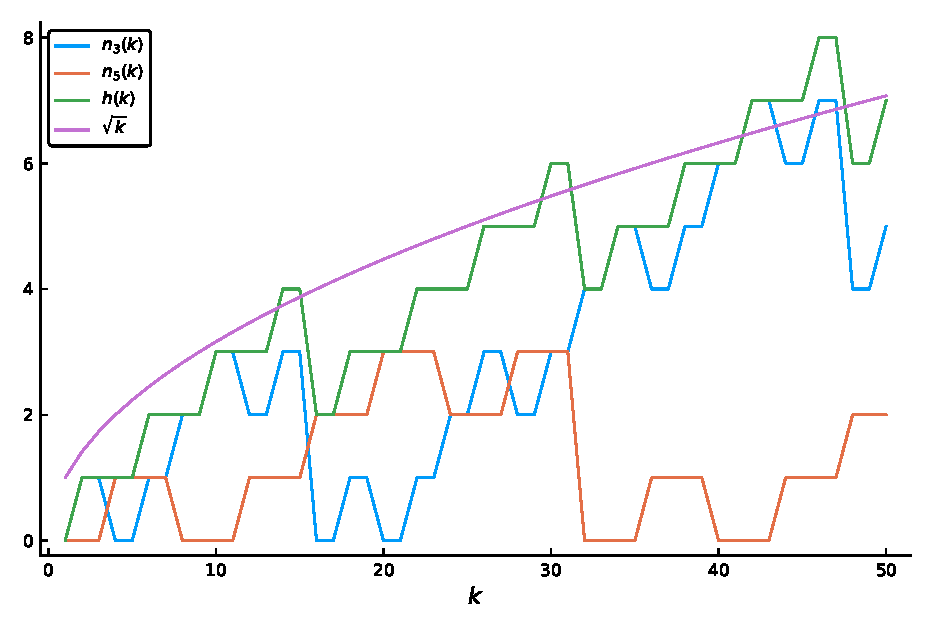
\includegraphics{behaviour_up_to_50}
\end{center}
\paragraph{Range $0$ to $5*10^2$}
\begin{center}
	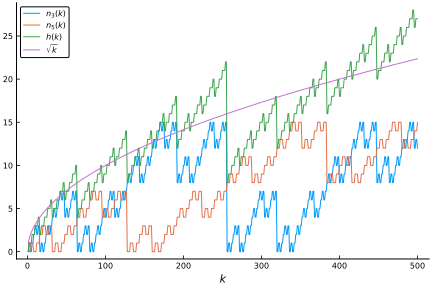
\includegraphics{behaviour_up_to_500}
\end{center}
\newpage
\paragraph{Range $0$ to $5*10^4$}
\begin{center}
	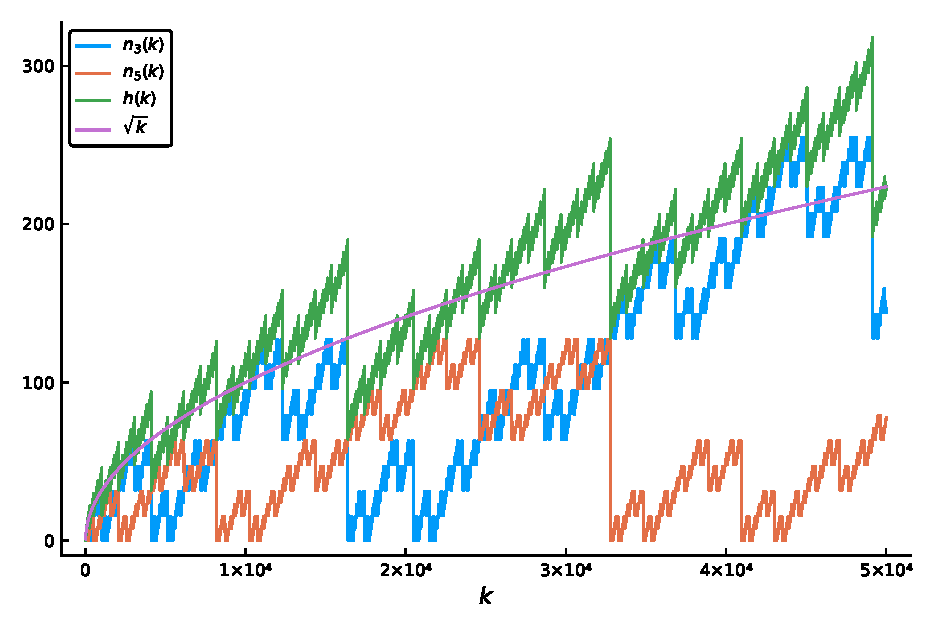
\includegraphics{behaviour_up_to_50000}
\end{center}
\paragraph{Range $0$ to $5*10^7$}
\begin{center}
	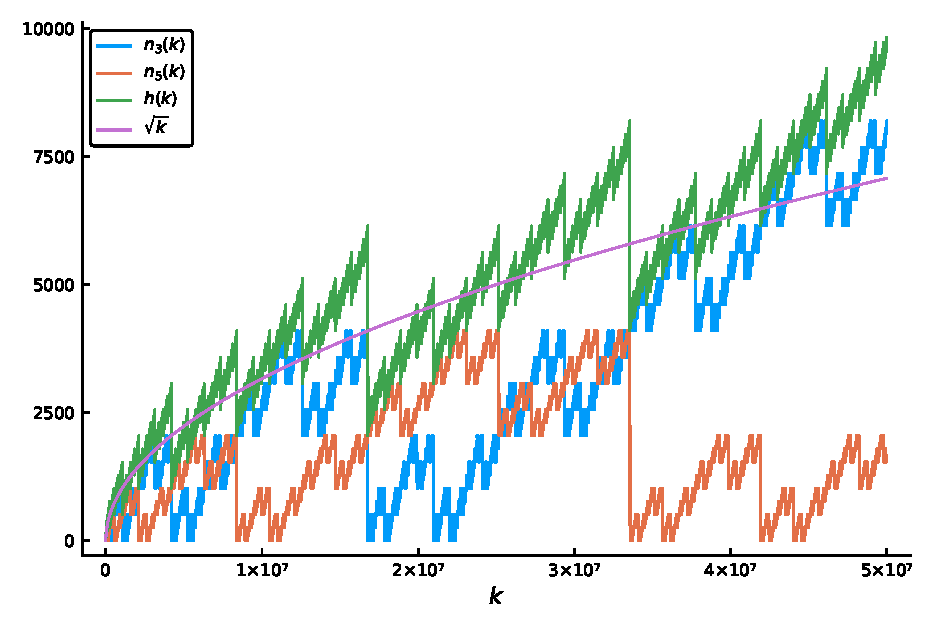
\includegraphics{behaviour_up_to_50000000}
\end{center}
Other pictures (including animated ones) may be found \href{https://pauldubois98.github.io/HeckeOperatorsModuloTwo/behaviour_h/}{online} at \url{https://pauldubois98.github.io/HeckeOperatorsModuloTwo/behaviour_h/}.



\newpage
\paragraph{Integers with Small Code}
\subparagraph{Table}
\label{table:CodeToIntegers}
As the codes of integers are in bijection with even numbers (or odd numbers), we can also plot even (or odd) integers as function of their code.
\begin{center}
	\begin{tabular}{|c||c|c|c|c|c|c|c|c|c|c|c|c|c|c|c|c|}
		\hline
		\textbf{} & \textbf{0} & \textbf{1} & \textbf{2} & \textbf{3} & \textbf{4} & \textbf{5} & \textbf{6} & \textbf{7} & \textbf{8} & \textbf{9} & \textbf{10} & \textbf{11} & \textbf{12} & \textbf{13} & \textbf{14} & \textbf{15} \\
		\hline\hline
		\textbf{0} & 0 & 4 & 16 & 20 & 64 & 68 & 80 & 84 & 256 & 260 & 272 & 276 & 320 & 324 & 336 & 340 \\
		\textbf{1} & 2 & 6 & 18 & 22 & 66 & 70 & 82 & 86 & 258 & 262 & 274 & 278 & 322 & 326 & 338 & 342 \\
		\textbf{2} & 8 & 12 & 24 & 28 & 72 & 76 & 88 & 92 & 264 & 268 & 280 & 284 & 328 & 332 & 344 & 348 \\
		\textbf{3} & 10 & 14 & 26 & 30 & 74 & 78 & 90 & 94 & 266 & 270 & 282 & 286 & 330 & 334 & 346 & 350 \\
		\textbf{4} & 32 & 36 & 48 & 52 & 96 & 100 & 112 & 116 & 288 & 292 & 304 & 308 & 352 & 356 & 368 & 372 \\
		\textbf{5} & 34 & 38 & 50 & 54 & 98 & 102 & 114 & 118 & 290 & 294 & 306 & 310 & 354 & 358 & 370 & 374 \\
		\textbf{6} & 40 & 44 & 56 & 60 & 104 & 108 & 120 & 124 & 296 & 300 & 312 & 316 & 360 & 364 & 376 & 380 \\
		\textbf{7} & 42 & 46 & 58 & 62 & 106 & 110 & 122 & 126 & 298 & 302 & 314 & 318 & 362 & 366 & 378 & 382 \\
		\textbf{8} & 128 & 132 & 144 & 148 & 192 & 196 & 208 & 212 & 384 & 388 & 400 & 404 & 448 & 452 & 464 & 468 \\
		\textbf{9} & 130 & 134 & 146 & 150 & 194 & 198 & 210 & 214 & 386 & 390 & 402 & 406 & 450 & 454 & 466 & 470 \\
		\textbf{10} & 136 & 140 & 152 & 156 & 200 & 204 & 216 & 220 & 392 & 396 & 408 & 412 & 456 & 460 & 472 & 476 \\
		%\textbf{11} & 138 & 142 & 154 & 158 & 202 & 206 & 218 & 222 & 394 & 398 & 410 & 414 & 458 & 462 & 474 & 478 \\
		%\textbf{12} & 160 & 164 & 176 & 180 & 224 & 228 & 240 & 244 & 416 & 420 & 432 & 436 & 480 & 484 & 496 & 500 \\
		%\textbf{13} & 162 & 166 & 178 & 182 & 226 & 230 & 242 & 246 & 418 & 422 & 434 & 438 & 482 & 486 & 498 & 502 \\
		%\textbf{14} & 168 & 172 & 184 & 188 & 232 & 236 & 248 & 252 & 424 & 428 & 440 & 444 & 488 & 492 & 504 & 508 \\
		%\textbf{15} & 170 & 174 & 186 & 190 & 234 & 238 & 250 & 254 & 426 & 430 & 442 & 446 & 490 & 494 & 506 & 510 \\
		\hline
	\end{tabular}
\end{center}
A larger table may be found \href{https://pauldubois98.github.io/HeckeOperatorsModuloTwo/code_to_even/}{online} at \url{https://pauldubois98.github.io/HeckeOperatorsModuloTwo/code_to_even/}.
Note that the same table may be produced for odd integers, find it  \href{https://pauldubois98.github.io/HeckeOperatorsModuloTwo/code_to_odd/}{online} at \url{https://pauldubois98.github.io/HeckeOperatorsModuloTwo/code_to_odd/}.



\subparagraph{Plots}
\label{plot:CodeSurface}
We plot the surface $z = \left[ x, y \right]$ i.e. $z$ is the integer with code $\left[ x, y \right]$.
\begin{center}
	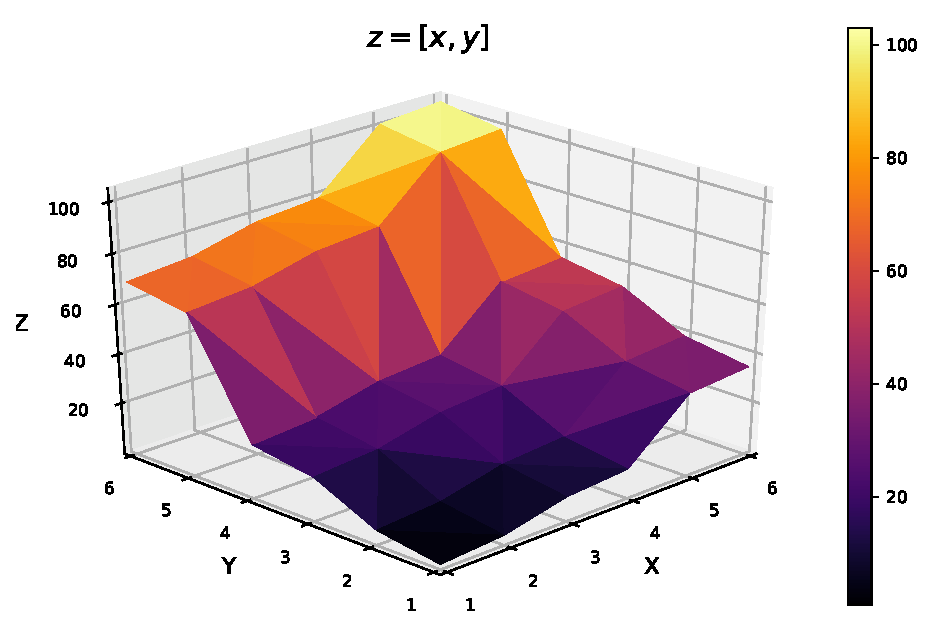
\includegraphics{code_plot_5-5}
\end{center}
\begin{center}
	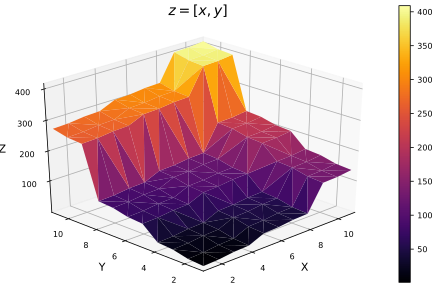
\includegraphics{code_plot_10-10}
\end{center}
\begin{center}
	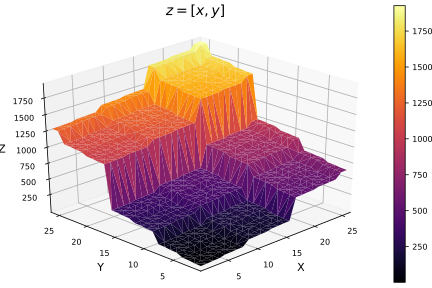
\includegraphics{code_plot_25-25}
\end{center}
Other pictures (including animated ones) may be found \href{https://pauldubois98.github.io/HeckeOperatorsModuloTwo/plot_code_to_int/}{online} at \url{https://pauldubois98.github.io/HeckeOperatorsModuloTwo/plot_code_to_int/}.



\newgeometry{margin=0.5cm, top=2cm, bottom=2cm}
\paragraph{Powers of $T_3$ and $T_5$ giving $\Delta^1$}
\label{table:OperatorToDelta1}
Here, wee look at the power of $\Delta^k$ such that when $T_3^aT_5^b$ is applied to it, we have $T_3^aT_5^b|\Delta^k = \Delta^1$.
\begin{center}
	\begin{tabular}{|c||c|c|c|c|c|c|c|c|c|c|c|c|c|c|c|}
		\hline
		\textbf{} & \textbf{$T_5^{0}$} & \textbf{$T_5^{1}$} & \textbf{$T_5^{2}$} & \textbf{$T_5^{3}$} & \textbf{$T_5^{4}$} & \textbf{$T_5^{5}$} & \textbf{$T_5^{6}$} & \textbf{$T_5^{7}$} & \textbf{$T_5^{8}$} & \textbf{$T_5^{9}$} & \textbf{$T_5^{10}$} & \textbf{$T_5^{11}$} & \textbf{$T_5^{12}$} & \textbf{$T_5^{13}$} & \textbf{$T_5^{14}$} \\
		\hline\hline
		$T_3^{0}$ & $\Delta^{1}$ & $\Delta^{5}$ & $\Delta^{17}$ & $\Delta^{21}$ & $\Delta^{65}$ & $\Delta^{69}$ & $\Delta^{81}$ & $\Delta^{85}$ & $\Delta^{257}$ & $\Delta^{261}$ & $\Delta^{273}$ & $\Delta^{277}$ & $\Delta^{321}$ & $\Delta^{325}$ & $\Delta^{337}$ \\
		$T_3^{1}$ & $\Delta^{3}$ & $\Delta^{7}$ & $\Delta^{19}$ & $\Delta^{23}$ & $\Delta^{67}$ & $\Delta^{71}$ & $\Delta^{83}$ & $\Delta^{87}$ & $\Delta^{259}$ & $\Delta^{263}$ & $\Delta^{275}$ & $\Delta^{279}$ & $\Delta^{323}$ & $\Delta^{327}$ & $\Delta^{339}$ \\
		$T_3^{2}$ & $\Delta^{9}$ & $\Delta^{13}$ & $\Delta^{25}$ & $\Delta^{29}$ & $\Delta^{73}$ & $\Delta^{77}$ & $\Delta^{89}$ & $\Delta^{93}$ & $\Delta^{265}$ & $\Delta^{269}$ & $\Delta^{281}$ & $\Delta^{285}$ & $\Delta^{329}$ & $\Delta^{333}$ & $\Delta^{345}$ \\
		$T_3^{3}$ & $\Delta^{11}$ & $\Delta^{15}$ & $\Delta^{27}$ & $\Delta^{31}$ & $\Delta^{75}$ & $\Delta^{79}$ & $\Delta^{91}$ & $\Delta^{95}$ & $\Delta^{267}$ & $\Delta^{271}$ & $\Delta^{283}$ & $\Delta^{287}$ & $\Delta^{331}$ & $\Delta^{335}$ & $\Delta^{347}$ \\
		$T_3^{4}$ & $\Delta^{33}$ & $\Delta^{37}$ & $\Delta^{49}$ & $\Delta^{53}$ & $\Delta^{97}$ & $\Delta^{101}$ & $\Delta^{113}$ & $\Delta^{117}$ 
		& $\Delta^{289}$ & $\Delta^{293}$ & $\Delta^{305}$ & $\Delta^{309}$ & $\Delta^{353}$ & $\Delta^{357}$ & $\Delta^{369}$ \\
		$T_3^{5}$ & $\Delta^{35}$ & $\Delta^{39}$ & $\Delta^{51}$ & $\Delta^{55}$ & $\Delta^{99}$ & $\Delta^{103}$ & $\Delta^{115}$ & $\Delta^{119}$ 
		& $\Delta^{291}$ & $\Delta^{295}$ & $\Delta^{307}$ & $\Delta^{311}$ & $\Delta^{355}$ & $\Delta^{359}$ & $\Delta^{371}$ \\
		$T_3^{6}$ & $\Delta^{41}$ & $\Delta^{45}$ & $\Delta^{57}$ & $\Delta^{61}$ & $\Delta^{105}$ & $\Delta^{109}$ & $\Delta^{121}$ & $\Delta^{125}$ & $\Delta^{297}$ & $\Delta^{301}$ & $\Delta^{313}$ & $\Delta^{317}$ & $\Delta^{361}$ & $\Delta^{365}$ & $\Delta^{377}$ \\
		$T_3^{7}$ & $\Delta^{43}$ & $\Delta^{47}$ & $\Delta^{59}$ & $\Delta^{63}$ & $\Delta^{107}$ & $\Delta^{111}$ & $\Delta^{123}$ & $\Delta^{127}$ & $\Delta^{299}$ & $\Delta^{303}$ & $\Delta^{315}$ & $\Delta^{319}$ & $\Delta^{363}$ & $\Delta^{367}$ & $\Delta^{379}$ \\
		$T_3^{8}$ & $\Delta^{129}$ & $\Delta^{133}$ & $\Delta^{145}$ & $\Delta^{149}$ & $\Delta^{193}$ & $\Delta^{197}$ & $\Delta^{209}$ & $\Delta^{213}$ & $\Delta^{385}$ & $\Delta^{389}$ & $\Delta^{401}$ & $\Delta^{405}$ & $\Delta^{449}$ & $\Delta^{453}$ & $\Delta^{465}$ \\
		$T_3^{9}$ & $\Delta^{131}$ & $\Delta^{135}$ & $\Delta^{147}$ & $\Delta^{151}$ & $\Delta^{195}$ & $\Delta^{199}$ & $\Delta^{211}$ & $\Delta^{215}$ & $\Delta^{387}$ & $\Delta^{391}$ & $\Delta^{403}$ & $\Delta^{407}$ & $\Delta^{451}$ & $\Delta^{455}$ & $\Delta^{467}$ \\
		$T_3^{10}$ & $\Delta^{137}$ & $\Delta^{141}$ & $\Delta^{153}$ & $\Delta^{157}$ & $\Delta^{201}$ & $\Delta^{205}$ & $\Delta^{217}$ & $\Delta^{221}$ & $\Delta^{393}$ & $\Delta^{397}$ & $\Delta^{409}$ & $\Delta^{413}$ & $\Delta^{457}$ & $\Delta^{461}$ & $\Delta^{473}$ \\
		$T_3^{11}$ & $\Delta^{139}$ & $\Delta^{143}$ & $\Delta^{155}$ & $\Delta^{159}$ & $\Delta^{203}$ & $\Delta^{207}$ & $\Delta^{219}$ & $\Delta^{223}$ & $\Delta^{395}$ & $\Delta^{399}$ & $\Delta^{411}$ & $\Delta^{415}$ & $\Delta^{459}$ & $\Delta^{463}$ & $\Delta^{475}$ \\
		$T_3^{12}$ & $\Delta^{161}$ & $\Delta^{165}$ & $\Delta^{177}$ & $\Delta^{181}$ & $\Delta^{225}$ & $\Delta^{229}$ & $\Delta^{241}$ & $\Delta^{245}$ & $\Delta^{417}$ & $\Delta^{421}$ & $\Delta^{433}$ & $\Delta^{437}$ & $\Delta^{481}$ & $\Delta^{485}$ & $\Delta^{497}$ \\
		$T_3^{13}$ & $\Delta^{163}$ & $\Delta^{167}$ & $\Delta^{179}$ & $\Delta^{183}$ & $\Delta^{227}$ & $\Delta^{231}$ & $\Delta^{243}$ & $\Delta^{247}$ & $\Delta^{419}$ & $\Delta^{423}$ & $\Delta^{435}$ & $\Delta^{439}$ & $\Delta^{483}$ & $\Delta^{487}$ & $\Delta^{499}$ \\
		$T_3^{14}$ & $\Delta^{169}$ & $\Delta^{173}$ & $\Delta^{185}$ & $\Delta^{189}$ & $\Delta^{233}$ & $\Delta^{237}$ & $\Delta^{249}$ & $\Delta^{253}$ & $\Delta^{425}$ & $\Delta^{429}$ & $\Delta^{441}$ & $\Delta^{445}$ & $\Delta^{489}$ & $\Delta^{493}$ & $\Delta^{505}$ \\
		$T_3^{15}$ & $\Delta^{171}$ & $\Delta^{175}$ & $\Delta^{187}$ & $\Delta^{191}$ & $\Delta^{235}$ & $\Delta^{239}$ & $\Delta^{251}$ & $\Delta^{255}$ & $\Delta^{427}$ & $\Delta^{431}$ & $\Delta^{443}$ & $\Delta^{447}$ & $\Delta^{491}$ & $\Delta^{495}$ & $\Delta^{507}$ \\
		$T_3^{16}$ & $\Delta^{513}$ & $\Delta^{517}$ & $\Delta^{529}$ & $\Delta^{533}$ & $\Delta^{577}$ & $\Delta^{581}$ & $\Delta^{593}$ & $\Delta^{597}$ & $\Delta^{769}$ & $\Delta^{773}$ & $\Delta^{785}$ & $\Delta^{789}$ & $\Delta^{833}$ & $\Delta^{837}$ & $\Delta^{849}$ \\
		$T_3^{17}$ & $\Delta^{515}$ & $\Delta^{519}$ & $\Delta^{531}$ & $\Delta^{535}$ & $\Delta^{579}$ & $\Delta^{583}$ & $\Delta^{595}$ & $\Delta^{599}$ & $\Delta^{771}$ & $\Delta^{775}$ & $\Delta^{787}$ & $\Delta^{791}$ & $\Delta^{835}$ & $\Delta^{839}$ & $\Delta^{851}$ \\
		$T_3^{18}$ & $\Delta^{521}$ & $\Delta^{525}$ & $\Delta^{537}$ & $\Delta^{541}$ & $\Delta^{585}$ & $\Delta^{589}$ & $\Delta^{601}$ & $\Delta^{605}$ & $\Delta^{777}$ & $\Delta^{781}$ & $\Delta^{793}$ & $\Delta^{797}$ & $\Delta^{841}$ & $\Delta^{845}$ & $\Delta^{857}$ \\
		$T_3^{19}$ & $\Delta^{523}$ & $\Delta^{527}$ & $\Delta^{539}$ & $\Delta^{543}$ & $\Delta^{587}$ & $\Delta^{591}$ & $\Delta^{603}$ & $\Delta^{607}$ & $\Delta^{779}$ & $\Delta^{783}$ & $\Delta^{795}$ & $\Delta^{799}$ & $\Delta^{843}$ & $\Delta^{847}$ & $\Delta^{859}$ \\
		$T_3^{20}$ & $\Delta^{545}$ & $\Delta^{549}$ & $\Delta^{561}$ & $\Delta^{565}$ & $\Delta^{609}$ & $\Delta^{613}$ & $\Delta^{625}$ & $\Delta^{629}$ & $\Delta^{801}$ & $\Delta^{805}$ & $\Delta^{817}$ & $\Delta^{821}$ & $\Delta^{865}$ & $\Delta^{869}$ & $\Delta^{881}$ \\
		$T_3^{21}$ & $\Delta^{547}$ & $\Delta^{551}$ & $\Delta^{563}$ & $\Delta^{567}$ & $\Delta^{611}$ & $\Delta^{615}$ & $\Delta^{627}$ & $\Delta^{631}$ & $\Delta^{803}$ & $\Delta^{807}$ & $\Delta^{819}$ & $\Delta^{823}$ & $\Delta^{867}$ & $\Delta^{871}$ & $\Delta^{883}$ \\
		$T_3^{22}$ & $\Delta^{553}$ & $\Delta^{557}$ & $\Delta^{569}$ & $\Delta^{573}$ & $\Delta^{617}$ & $\Delta^{621}$ & $\Delta^{633}$ & $\Delta^{637}$ & $\Delta^{809}$ & $\Delta^{813}$ & $\Delta^{825}$ & $\Delta^{829}$ & $\Delta^{873}$ & $\Delta^{877}$ & $\Delta^{889}$ \\
		$T_3^{23}$ & $\Delta^{555}$ & $\Delta^{559}$ & $\Delta^{571}$ & $\Delta^{575}$ & $\Delta^{619}$ & $\Delta^{623}$ & $\Delta^{635}$ & $\Delta^{639}$ & $\Delta^{811}$ & $\Delta^{815}$ & $\Delta^{827}$ & $\Delta^{831}$ & $\Delta^{875}$ & $\Delta^{879}$ & $\Delta^{891}$ \\
		$T_3^{24}$ & $\Delta^{641}$ & $\Delta^{645}$ & $\Delta^{657}$ & $\Delta^{661}$ & $\Delta^{705}$ & $\Delta^{709}$ & $\Delta^{721}$ & $\Delta^{725}$ & $\Delta^{897}$ & $\Delta^{901}$ & $\Delta^{913}$ & $\Delta^{917}$ & $\Delta^{961}$ & $\Delta^{965}$ & $\Delta^{977}$ \\
		$T_3^{25}$ & $\Delta^{643}$ & $\Delta^{647}$ & $\Delta^{659}$ & $\Delta^{663}$ & $\Delta^{707}$ & $\Delta^{711}$ & $\Delta^{723}$ & $\Delta^{727}$ & $\Delta^{899}$ & $\Delta^{903}$ & $\Delta^{915}$ & $\Delta^{919}$ & $\Delta^{963}$ & $\Delta^{967}$ & $\Delta^{979}$ \\
		$T_3^{26}$ & $\Delta^{649}$ & $\Delta^{653}$ & $\Delta^{665}$ & $\Delta^{669}$ & $\Delta^{713}$ & $\Delta^{717}$ & $\Delta^{729}$ & $\Delta^{733}$ & $\Delta^{905}$ & $\Delta^{909}$ & $\Delta^{921}$ & $\Delta^{925}$ & $\Delta^{969}$ & $\Delta^{973}$ & $\Delta^{985}$ \\
		$T_3^{27}$ & $\Delta^{651}$ & $\Delta^{655}$ & $\Delta^{667}$ & $\Delta^{671}$ & $\Delta^{715}$ & $\Delta^{719}$ & $\Delta^{731}$ & $\Delta^{735}$ & $\Delta^{907}$ & $\Delta^{911}$ & $\Delta^{923}$ & $\Delta^{927}$ & $\Delta^{971}$ & $\Delta^{975}$ & $\Delta^{987}$ \\
		$T_3^{28}$ & $\Delta^{673}$ & $\Delta^{677}$ & $\Delta^{689}$ & $\Delta^{693}$ & $\Delta^{737}$ & $\Delta^{741}$ & $\Delta^{753}$ & $\Delta^{757}$ & $\Delta^{929}$ & $\Delta^{933}$ & $\Delta^{945}$ & $\Delta^{949}$ & $\Delta^{993}$ & $\Delta^{997}$ & $\Delta^{1009}$ \\
		$T_3^{29}$ & $\Delta^{675}$ & $\Delta^{679}$ & $\Delta^{691}$ & $\Delta^{695}$ & $\Delta^{739}$ & $\Delta^{743}$ & $\Delta^{755}$ & $\Delta^{759}$ & $\Delta^{931}$ & $\Delta^{935}$ & $\Delta^{947}$ & $\Delta^{951}$ & $\Delta^{995}$ & $\Delta^{999}$ & $\Delta^{1011}$ \\
		$T_3^{30}$ & $\Delta^{681}$ & $\Delta^{685}$ & $\Delta^{697}$ & $\Delta^{701}$ & $\Delta^{745}$ & $\Delta^{749}$ & $\Delta^{761}$ & $\Delta^{765}$ & $\Delta^{937}$ & $\Delta^{941}$ & $\Delta^{953}$ & $\Delta^{957}$ & $\Delta^{1001}$ & $\Delta^{1005}$ & $\Delta^{1017}$ \\
		\hline
	\end{tabular}
\end{center}
A larger table may be found \href{https://pauldubois98.github.io/HeckeOperatorsModuloTwo/T3T5_powers_to_delta/}{online} at \url{https://pauldubois98.github.io/HeckeOperatorsModuloTwo/T3T5_powers_to_delta/}.



\newgeometry{margin=2cm}
\subsection{Behaviour of $h$ on Various Scales}
\label{expansionsOfTp}
Here are expansions of $T_p$ in series of $T_3^aT_5^b$ for primes $p<80$:\\
$T_{3} = T_3^{1}T_5^{0}$\\
$T_{5} = T_3^{0}T_5^{1}$\\
$T_{7} = T_3^{1}T_5^{1} + T_3^{3}T_5^{1} + T_3^{3}T_5^{3} + T_3^{5}T_5^{1} + T_3^{1}T_5^{7} + T_3^{1}T_5^{9} + T_3^{7}T_5^{3} + T_3^{7}T_5^{5} + T_3^{9}T_5^{3} + T_3^{11}T_5^{1} + T_3^{3}T_5^{11} + T_3^{5}T_5^{9} + T_3^{13}T_5^{1} + T_3^{3}T_5^{13} + T_3^{5}T_5^{11} + T_3^{9}T_5^{7} + T_3^{11}T_5^{5} + T_3^{13}T_5^{3} + T_3^{3}T_5^{15} + T_3^{7}T_5^{11} + T_3^{9}T_5^{9} + T_3^{13}T_5^{5} + T_3^{15}T_5^{3} + \dots $\\   
$T_{11} = T_3^{1}T_5^{0} + T_3^{1}T_5^{2} + T_3^{3}T_5^{0} + T_3^{1}T_5^{4} + T_3^{3}T_5^{2} + T_3^{5}T_5^{0} + T_3^{1}T_5^{6} + T_3^{3}T_5^{4} + T_3^{7}T_5^{2} + T_3^{1}T_5^{10} + T_3^{3}T_5^{8} + T_3^{7}T_5^{4} + T_3^{9}T_5^{2} + T_3^{11}T_5^{2} + T_3^{3}T_5^{12} + T_3^{5}T_5^{10} + T_3^{7}T_5^{8} + T_3^{11}T_5^{4} + T_3^{13}T_5^{2} + T_3^{9}T_5^{8} + T_3^{17}T_5^{0} + \dots $\\
$T_{13} = T_3^{0}T_5^{1} + T_3^{0}T_5^{3} + T_3^{2}T_5^{1} + T_3^{0}T_5^{5} + T_3^{4}T_5^{1} + T_3^{2}T_5^{5} + T_3^{4}T_5^{3} + T_3^{6}T_5^{1} + T_3^{0}T_5^{9} + T_3^{2}T_5^{7} + T_3^{6}T_5^{3} + T_3^{0}T_5^{11} + T_3^{6}T_5^{5} + T_3^{8}T_5^{3} + T_3^{10}T_5^{1} + T_3^{2}T_5^{11} + T_3^{4}T_5^{9} + T_3^{6}T_5^{7} + T_3^{10}T_5^{3} + T_3^{2}T_5^{13} + T_3^{4}T_5^{11} + T_3^{14}T_5^{1} + T_3^{2}T_5^{15} + T_3^{4}T_5^{13} + T_3^{6}T_5^{11} + T_3^{12}T_5^{5} + T_3^{16}T_5^{1} + \dots $\\
$T_{17} = T_3^{0}T_5^{2} + T_3^{2}T_5^{0} + T_3^{2}T_5^{2} + T_3^{0}T_5^{6} + T_3^{4}T_5^{2} + T_3^{6}T_5^{0} + T_3^{2}T_5^{6} + T_3^{4}T_5^{4} + T_3^{6}T_5^{2} + T_3^{10}T_5^{0} + T_3^{2}T_5^{10} + T_3^{4}T_5^{8} + T_3^{6}T_5^{6} + T_3^{10}T_5^{2} + T_3^{2}T_5^{12} + T_3^{6}T_5^{8} + T_3^{10}T_5^{4} + T_3^{2}T_5^{14} + T_3^{6}T_5^{10} + T_3^{8}T_5^{8} + T_3^{12}T_5^{4} + T_3^{14}T_5^{2} + T_3^{4}T_5^{14} + T_3^{8}T_5^{10} + T_3^{10}T_5^{8} + T_3^{12}T_5^{6} + T_3^{16}T_5^{2} + T_3^{18}T_5^{0} + \dots $\\
$T_{19} = T_3^{1}T_5^{0} + T_3^{3}T_5^{0} + T_3^{1}T_5^{4} + T_3^{3}T_5^{2} + T_3^{1}T_5^{6} + T_3^{5}T_5^{2} + T_3^{3}T_5^{6} + T_3^{7}T_5^{2} + T_3^{9}T_5^{0} + T_3^{1}T_5^{10} + T_3^{7}T_5^{4} + T_3^{9}T_5^{2} + T_3^{11}T_5^{0} + T_3^{1}T_5^{12} + T_3^{5}T_5^{8} + T_3^{11}T_5^{2} + T_3^{13}T_5^{0} + T_3^{3}T_5^{12} + T_3^{7}T_5^{8} + T_3^{9}T_5^{6} + T_3^{11}T_5^{4} + T_3^{13}T_5^{2} + T_3^{3}T_5^{14} + T_3^{7}T_5^{10} + T_3^{11}T_5^{6} + T_3^{15}T_5^{2} + T_3^{17}T_5^{0} + \dots $\\
$T_{23} = T_3^{1}T_5^{1} + T_3^{1}T_5^{3} + T_3^{5}T_5^{1} + T_3^{1}T_5^{7} + T_3^{5}T_5^{5} + T_3^{7}T_5^{3} + T_3^{1}T_5^{13} + T_3^{5}T_5^{9} + T_3^{7}T_5^{7} + T_3^{1}T_5^{15} + T_3^{3}T_5^{13} + T_3^{5}T_5^{11} + T_3^{7}T_5^{9} + T_3^{11}T_5^{5} + T_3^{13}T_5^{3} + T_3^{15}T_5^{1} + T_3^{17}T_5^{1} + \dots $\\
$T_{29} = T_3^{0}T_5^{1} + T_3^{0}T_5^{3} + T_3^{2}T_5^{3} + T_3^{2}T_5^{5} + T_3^{6}T_5^{1} + T_3^{0}T_5^{9} + T_3^{0}T_5^{11} + T_3^{2}T_5^{9} + T_3^{4}T_5^{7} + T_3^{8}T_5^{3} + T_3^{0}T_5^{13} + T_3^{6}T_5^{7} + T_3^{10}T_5^{3} + T_3^{12}T_5^{1} + T_3^{2}T_5^{13} + T_3^{8}T_5^{7} + T_3^{4}T_5^{13} + T_3^{6}T_5^{11} + T_3^{12}T_5^{5} + T_3^{14}T_5^{3} + T_3^{16}T_5^{1} + \dots $\\
$T_{31} = T_3^{1}T_5^{1} + T_3^{1}T_5^{3} + T_3^{3}T_5^{3} + T_3^{5}T_5^{1} + T_3^{3}T_5^{5} + T_3^{1}T_5^{9} + T_3^{1}T_5^{11} + T_3^{9}T_5^{3} + T_3^{11}T_5^{1} + T_3^{1}T_5^{13} + T_3^{3}T_5^{11} + T_3^{9}T_5^{5} + T_3^{1}T_5^{15} + T_3^{9}T_5^{7} + T_3^{15}T_5^{1} + T_3^{13}T_5^{5} + T_3^{15}T_5^{3} + \dots $\\
$T_{37} = T_3^{0}T_5^{1} + T_3^{0}T_5^{3} + T_3^{2}T_5^{1} + T_3^{2}T_5^{3} + T_3^{2}T_5^{5} + T_3^{4}T_5^{3} + T_3^{2}T_5^{7} + T_3^{6}T_5^{3} + T_3^{8}T_5^{1} + T_3^{6}T_5^{5} + T_3^{2}T_5^{11} + T_3^{6}T_5^{7} + T_3^{8}T_5^{5} + T_3^{12}T_5^{1} + T_3^{6}T_5^{9} + T_3^{8}T_5^{7} 
+ T_3^{2}T_5^{15} + T_3^{4}T_5^{13} + T_3^{12}T_5^{5} + \dots $\\
$T_{41} = T_3^{0}T_5^{2} + T_3^{2}T_5^{2} + T_3^{4}T_5^{0} + T_3^{2}T_5^{4} + T_3^{4}T_5^{2} + T_3^{6}T_5^{2} + T_3^{0}T_5^{10} + T_3^{2}T_5^{10} + T_3^{8}T_5^{4} + T_3^{10}T_5^{2} + T_3^{12}T_5^{0} + T_3^{0}T_5^{14} + T_3^{2}T_5^{12} + T_3^{8}T_5^{6} + T_3^{14}T_5^{2} + T_3^{4}T_5^{14} + T_3^{8}T_5^{10} + T_3^{10}T_5^{8} + T_3^{16}T_5^{2} + \dots $\\
$T_{43} = T_3^{1}T_5^{0} + T_3^{3}T_5^{2} + T_3^{5}T_5^{0} + T_3^{1}T_5^{6} + T_3^{3}T_5^{4} + T_3^{5}T_5^{2} + T_3^{7}T_5^{0} + T_3^{7}T_5^{2} + T_3^{5}T_5^{6} + T_3^{9}T_5^{2} + T_3^{5}T_5^{8} + T_3^{9}T_5^{4} + T_3^{3}T_5^{12} + T_3^{5}T_5^{10} + T_3^{9}T_5^{6} + T_3^{11}T_5^{4} + T_3^{3}T_5^{14} + T_3^{5}T_5^{12} + T_3^{9}T_5^{8} + T_3^{11}T_5^{6} + T_3^{13}T_5^{4} + \dots $\\
$T_{47} = T_3^{1}T_5^{1} + T_3^{1}T_5^{5} + T_3^{3}T_5^{3} + T_3^{5}T_5^{1} + T_3^{5}T_5^{3} + T_3^{3}T_5^{7} + T_3^{5}T_5^{5} + T_3^{9}T_5^{1} + T_3^{1}T_5^{11} + T_3^{5}T_5^{7} + T_3^{7}T_5^{5} + T_3^{1}T_5^{13} + T_3^{5}T_5^{9} + T_3^{9}T_5^{5} + T_3^{3}T_5^{13} + T_3^{9}T_5^{7} + T_3^{11}T_5^{5} + T_3^{13}T_5^{3} + T_3^{15}T_5^{1} + T_3^{3}T_5^{15} + T_3^{7}T_5^{11} + T_3^{9}T_5^{9} + T_3^{15}T_5^{3} + \dots $\\    
$T_{53} = T_3^{0}T_5^{1} + T_3^{2}T_5^{1} + T_3^{0}T_5^{5} + T_3^{2}T_5^{3} + T_3^{4}T_5^{1} + T_3^{0}T_5^{7} + T_3^{4}T_5^{3} + T_3^{6}T_5^{1} + T_3^{0}T_5^{9} + T_3^{4}T_5^{5} + T_3^{8}T_5^{1} + T_3^{10}T_5^{1} + T_3^{8}T_5^{5} + T_3^{2}T_5^{13} + T_3^{4}T_5^{11} + T_3^{6}T_5^{9} + T_3^{10}T_5^{5} + T_3^{14}T_5^{1} + T_3^{2}T_5^{15} + T_3^{4}T_5^{13} + T_3^{6}T_5^{11} + T_3^{14}T_5^{3} + T_3^{16}T_5^{1} + \dots $\\   
$T_{59} = T_3^{1}T_5^{0} + T_3^{1}T_5^{2} + T_3^{5}T_5^{0} + T_3^{1}T_5^{6} + T_3^{5}T_5^{2} + T_3^{7}T_5^{0} + T_3^{1}T_5^{8} + T_3^{9}T_5^{0} + T_3^{5}T_5^{6} + T_3^{7}T_5^{4} + T_3^{9}T_5^{2} + T_3^{3}T_5^{10} + T_3^{7}T_5^{6} + T_3^{5}T_5^{10} + T_3^{7}T_5^{8} + T_3^{9}T_5^{6} 
+ T_3^{9}T_5^{8} + T_3^{11}T_5^{6} + \dots $\\
$T_{61} = T_3^{0}T_5^{1} + T_3^{2}T_5^{1} + T_3^{0}T_5^{5} + T_3^{2}T_5^{3} + T_3^{0}T_5^{7} + T_3^{6}T_5^{3} + T_3^{8}T_5^{1} + T_3^{2}T_5^{9} + T_3^{4}T_5^{7} + T_3^{8}T_5^{3} + T_3^{2}T_5^{11} + T_3^{4}T_5^{9} + T_3^{10}T_5^{3} + T_3^{12}T_5^{1} + T_3^{4}T_5^{11} + T_3^{6}T_5^{9} + T_3^{12}T_5^{3} + T_3^{4}T_5^{13} + T_3^{6}T_5^{11} + T_3^{8}T_5^{9} + \dots $\\
$T_{67} = T_3^{1}T_5^{0} + T_3^{1}T_5^{2} + T_3^{3}T_5^{0} + T_3^{1}T_5^{4} + T_3^{5}T_5^{0} + T_3^{3}T_5^{4} + T_3^{3}T_5^{6} + T_3^{7}T_5^{2} + T_3^{9}T_5^{0} + T_3^{1}T_5^{10} + T_3^{3}T_5^{8} + T_3^{5}T_5^{6} + T_3^{9}T_5^{2} + T_3^{11}T_5^{0} + T_3^{3}T_5^{10} + T_3^{5}T_5^{8} + T_3^{7}T_5^{6} + T_3^{9}T_5^{4} + T_3^{1}T_5^{14} + T_3^{3}T_5^{12} + T_3^{5}T_5^{10} + T_3^{7}T_5^{8} + T_3^{9}T_5^{6} + T_3^{5}T_5^{12} 
+ T_3^{9}T_5^{8} + T_3^{11}T_5^{6} + T_3^{13}T_5^{4} + T_3^{15}T_5^{2} + \dots $\\
$T_{71} = T_3^{1}T_5^{1} + T_3^{1}T_5^{3} + T_3^{3}T_5^{5} + T_3^{7}T_5^{1} + T_3^{3}T_5^{7} + T_3^{5}T_5^{5} + T_3^{7}T_5^{5} + T_3^{9}T_5^{3} + T_3^{3}T_5^{11} + T_3^{7}T_5^{7} + T_3^{9}T_5^{5} + T_3^{11}T_5^{3} + T_3^{13}T_5^{1} + T_3^{3}T_5^{13} + T_3^{5}T_5^{11} + T_3^{9}T_5^{7} + T_3^{11}T_5^{5} + T_3^{13}T_5^{3} + T_3^{15}T_5^{1} + T_3^{7}T_5^{11} + T_3^{13}T_5^{5} + \dots $\\
$T_{73} = T_3^{2}T_5^{0} + T_3^{0}T_5^{4} + T_3^{2}T_5^{2} + T_3^{2}T_5^{4} + T_3^{6}T_5^{0} + T_3^{2}T_5^{6} + T_3^{2}T_5^{8} + T_3^{4}T_5^{6} + T_3^{8}T_5^{2} + T_3^{10}T_5^{2} + T_3^{4}T_5^{10} + T_3^{6}T_5^{8} + T_3^{8}T_5^{6} + T_3^{10}T_5^{4} + T_3^{2}T_5^{14} + T_3^{8}T_5^{8} + T_3^{10}T_5^{6} + T_3^{10}T_5^{8} + T_3^{16}T_5^{2} + \dots $\\
$T_{79} = T_3^{1}T_5^{1} + T_3^{1}T_5^{3} + T_3^{3}T_5^{1} + T_3^{1}T_5^{5} + T_3^{1}T_5^{7} + T_3^{7}T_5^{1} + T_3^{1}T_5^{9} + T_3^{7}T_5^{3} + T_3^{1}T_5^{11} + T_3^{9}T_5^{3} + T_3^{1}T_5^{13} + T_3^{3}T_5^{11} + T_3^{5}T_5^{9} + T_3^{7}T_5^{7} + T_3^{9}T_5^{5} + T_3^{11}T_5^{3} + T_3^{3}T_5^{13} + T_3^{7}T_5^{9} + T_3^{11}T_5^{5} + T_3^{15}T_5^{1} + T_3^{3}T_5^{15} + T_3^{5}T_5^{13} + T_3^{9}T_5^{9} + T_3^{11}T_5^{7} + \dots $\\
Expansions for larger primes may be found \href{https://pauldubois98.github.io/HeckeOperatorsModuloTwo/T_p_extensions/}{online} at \url{https://pauldubois98.github.io/HeckeOperatorsModuloTwo/T_p_extensions/}.


